\section{Output Variable Dos and Don'ts}\label{output-variable-dos-and-donts}

For general output variables there aren't many rules. For meter output variables there are quite a few. Here are some tips to keep you out of trouble.

\subsection{What Variables Should I Output?}\label{what-variables-should-i-output}

The choice of variables to output is really up to the developer. Since variables don't appear on the output file unless requested by the user in the IDF input file, it is better to ``SetUp'' too many rather than too few. For an HVAC component one should generally output the heating and cooling outputs of the component both in terms of energy and power. Energy is always output in Joules, power in Watts. If there is humidification or dehumidification both total and sensible cooling should be reported. Any electricity or fuel consumed by a component should be reported out, again both in terms of energy (Joules) and power (Watts). For HVAC components in most cases reporting inlet and outlet temperatures and humidities is unnecessary since these quantities can be obtained from the system node outputs.

\subsection{Output Variable Naming Conventions}\label{output-variable-naming-conventions}

The names for output variables need to be selected carefully to maintain a high level of consistency and clarity. Well-chosen names help users quickly understand the meaning of a specific output.

The following general guidelines are to be followed when choosing names for new output variables:

\begin{itemize}
\item
  Output variable names shall be written in title case where every major word is capitalized (exceptions: ``a'', ``the'', ``for'', etc.) with spaces separating words.
\item
  Output variable names shall be written using natural language terminology but should be relatively concise. The language is American English.
\item
  Although they should be avoided where practical, acronyms (and symbols) are acceptable where their use is commonplace and contributes to conciseness in identifying a complex engineering concept. Examples of acceptable acronyms for output variable names are listed in the table below.
\item
  Abbreviations should not be used and the words spelled out completely (except for Units).
\item
  Where practical, reuse existing names for output variables across different models for similar components.~ For example, a new model for a zone baseboard heater should reuse the existing names for output variables already in use for other baseboard models rather than use new names that distinguish the kind of baseboard model that the output is associated with.~ The user-defined name of the component should allow the user to know the association without the basic name of the output variable reflecting that association.~ This has the advantage of reducing the total number of output variable names and making it simpler for users.
\item
  Engineering terminology should generally be consistent with that used in ASHRAE handbooks and literature (American Society of Heating, Refrigeration and~ Air-Conditioning Engineers, Inc., Atlanta, CA, USA)
\item
  Output variable names shall have no punctuation or special characters. The names are expected to contain many adjectives adjacent to each other and no hyphens or commas are needed to clarify.
\item
  Output variable names shall always be less than 100 characters long.
\end{itemize}

An output variable name should be constructed from up to six separate name elements.~ The following diagram shows the elements and the order that they are to be used in the name.~ The first three are each somewhat optional and are used as needed to identify the type of engineering model, object, or device being reported on.~ The last three are nearly always needed. Units are always needed (as described below.

\begin{figure}[hbtp] % fig 2
\centering
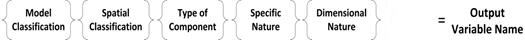
\includegraphics[width=0.9\textwidth, height=0.9\textheight, keepaspectratio=true]{media/image003.jpg}
\caption{Output Variable Classification Elements \protect \label{fig:output-variable-classification-elements}}
\end{figure}

\textbf{Model Classification}. This name element is used to identify the specific type of modeling being conducted.~ When used, it will form the first part of the name. This name element is often not needed, such as when the output is for a more or less usual aspect of buildings and HVAC system models.~ This is typically used to identify outputs that are associated with an alternative, usually more advanced, model, such as AirflowNetwork (AFN) or Conduction Finite Difference (CondFD).~ Although modeling domains such as Building, HVAC, or Internal Loads are usually obvious and not needed here, this classification can be useful for non-obvious sub-domains such as Environmental Impact, Refrigeration, or Daylighting.

\textbf{Spatial Classification}. This name element is used to identify spatial or topological location of the thing being reported on.~ It is generally used to identify which part of the building or system is being referred to by the output.~ For parts of the building, classifications such as ``Zone'' and ``Surface'' are the most common.~ For a model such as Refrigeration this classification may identify specific parts of the system, such as ``Secondary Loop.''~ There is often no spatial or topological aspect needed and in that case this name element can be omitted.

\textbf{Type of Component}. This name element is used to identify the type of device or phenomena being modeled and reported on.~ For most component models this should be a simple generic term for the type of device and attempt to reuse established names for similar devices or models.~ In cases where the Model and Spatial Classifications are sufficient, this element can be omitted.

\textbf{Specific Nature.} This name element is used to identify the nature of what is being reported for the device or phenomena being modeled. This is where the most low-level and specific detail is applied to describe the output variable.~ This name element is nearly always needed.

\textbf{Dimensional Nature.} This name element is used to identify the nature of the physical dimensions of the quantity being reported in words.~ This name element is nearly always needed. This name element is the final part of the name so that names end with terms that reflect the nature of the value being reported. However, the name element should not be the actual units.~ For example, an output that has units of degrees Celsius, the final word in the name should be ``Temperature.''~ Or an output for air flow that has units of kg/s, the final words in the name should be ``Mass Flow Rate.''~ When reporting on electricity use in Watts, the term ``Power'' is used; however most other uses of Watts use the term ``Rate.''

\textbf{Units}. This name element is used to identify the units of the value being reported.~ ~Units of output variables are strictly SI, as used in EnergyPlus.~ Units are concatenated on the end of the name with square brackets and separated by a space and.~ Dimensionless quantities shall use empty brackets ``{[} {]}.''~ The preferred set of units is listed at the top of the Energy+.idd file. Units are always abbreviated.

In some situations, a model may lend itself to generating a series of related output variables that depend on input.~ For example a surface heat transfer model may have results for numerous individual nodes or cells across the thickness of the surfaces.~ The number of nodes in the model will vary at runtime depending on the Construction.~ When this is the case, the standard approach used in EnergyPlus is to produce a series of output variables by enumerating the output variable name (rather than the key value) to generate a specific name for each instance.~ The generated name element for each instance in the series is appended to the end of the name (but before the Units element) and should end in a number. For example, the third node in a stratified tank model is called ``Chilled Water Thermal Storage Temperature Node 3 {[}C{]}.''~ This is done to facilitate wildcarding when postprocessing output.

For Version 8.0, a comprehensive effort was made to rename output variables to follow the guidelines and scheme described above.~ As of Version 8.0 the existing output variables demonstrate the pattern and should serve as good examples to follow for future output variables. The following table lists a few examples of terms, but these are not meant to be comprehensive or restrictive.~ It is expected that new models may have valid reasons to introduce new terms and units. Developers should examine RDD output files for comprehensive lists of example output variable names.

% table 5
\begin{longtable}[c]{p{1.5in}p{1.5in}p{1.5in}p{1.5in}}
\caption{Output Variable Classifications \label{table:output-variable-classifications}} \tabularnewline
\toprule 
Model Classification & Spatial Classification & Type of Component & Dimensional Nature \tabularnewline
\midrule
\endfirsthead

\caption[]{Output Variable Classifications} \tabularnewline
\toprule 
Model Classification & Spatial Classification & Type of Component & Dimensional Nature \tabularnewline
\midrule
\endhead

AFN & Zone & Inside Face & Rate \tabularnewline
Refrigeration & Surface & Outside Face & Rate per Area \tabularnewline
Room Air & Linkage & Air Terminal & Energy \tabularnewline
HAMT & Interior & Boiler & Temperature \tabularnewline
CondFD & Exterior & Chiller & Mass Flow Rate \tabularnewline
EMPD & Site & Cooling Coil & COP \tabularnewline
Plant & Supply Side & Infiltration & Power (electric) \tabularnewline
Environmental Impact & Air System & Unit Heater & Level \tabularnewline
HVAC & Facility & Generator & Fraction \tabularnewline
Setpoint Manager & Node & Baseboard & Status \tabularnewline
\bottomrule
\end{longtable}

~The following table lists acronyms and symbols used in output variable names.

Table 6. Output Variable Example Abbreviations

Acronym

Definition

AC

Alternating Current

AFN

AirflowNetwork

Ar

Argon

ASHRAE

American Society of Heating, Refrigeration, and Air-Conditioning Engineers, Inc.

BSDF

Bidirectional Scattering Distribution Function

CEN

European Committee for Standardization (Comite Europeen de Normalisation)

CH4

Methane

CO

Carbon Monoxide

CO2

Carbon Dioxide

CondFD

Conduction Finite Difference

COP

Coefficient of Performance

DC

Direct Current

DX

Direct Expansion

EIR

Energy Input Ratio

EMPD

Effective Moisture Penetration Depth

H20

Water

HAMT

Heat and Moisture Transfer

Hg

Mercury

HHV

Higher Heating Value

HVAC

Heating Ventilation and Air Conditioning

KSU

Kansas State University

LHV

Lower Heating Value

N2

Nitrogen

N2O

Nitrous Oxide

NH3

Ammonia

NMVOC

Non-Methane Volatile Organic Compounds

NOx

Nitrogen Oxides

O2

Oxygen

Pb

Lead

PM

Particulate Matter

PM10

Particulate Matter of 10 microns or less in size

PM2.5

Particulate Matter of 2.5 microns or less in size

PMV

Predicted Mean Vote

PPD

Percent People Dissatisfied

PV

Photovoltaic

PVT

Photovoltaic-Thermal

SO2

Sulfur Dioxide

VAV

Variable Air Volume

VRF

Variable Refrigerant Flow

WAHP

Water to Air Heat Pump

\subsection{What are Meters?}\label{what-are-meters}

In EnergyPlus meters are an additional output reporting capability. A meter is a way of grouping similar output variables. Meters are output variables just like ordinary output variables except that they sum or average a collection of ordinary output variables. In EnergyPlus the meter variables serve two purposes.

\begin{itemize}
\item
  Providing output of fuel and electricity consumption by end use categories and at the system plant, building and facility level.
\item
  Providing a way of summing heating or cooling outputs for a category of components. The resource type EnergyTransfer is used for this purpose. An example would be reporting out the sum of the heating energy from all the heating coils in a system.
\end{itemize}

\subsection{How Do I Create A Meter?}\label{how-do-i-create-a-meter}

Meter output variables are created at the same time and in the same manner as ordinary output variables. SetupOutputVariable is called but the optional arguments ResourceTypeKey, EndUseKey, and GroupKey must be used in addition to the usual arguments. For example, in the electric steam humidifier module

CALL SetupOutputVariable(`Humidifier Electric Energy {[}J{]}', \&

~ Humidifier(HumNum)\%ElecUseEnergy, `System',`Sum', \&

~ Humidifier(HumNum)\%Name)

creates an output variable labeled `Humidifier Electric Energy {[}J{]}' with the value of Humidifier(HumNum)\%ElecUseEnergy.

CALL SetupOutputVariable(`Humidifier Electric Energy {[}J{]}', \&

~ Humidifier(HumNum)\%ElecUseEnergy, `System',`Sum', \&

~ Humidifier(HumNum)\%Name, \& ~ ResourceTypeKey = `ELECTRICITY',EndUseKey = `HUMIDIFIER', \&

~ GroupKey = `System')

Creates the same output variable but in addition creates a meter output variable Humidifier:Electricity {[}J{]}. This variable will contain the sum of all the electricity consumption of the humidifiers in the system. In addition, this electrical consumption will be added into the meter variables Electricity:HVAC {[}J{]} and Electricity:Facility {[}J{]}.

\subsection{Rules for Meter Variables}\label{rules-for-meter-variables}

There are a number of rules developers must follow in order to account for all electricity and fuel consumption as well as to prevent consumables from being double counted.

t~Electricity and fuel meters must always be defined at the simple component level. Some EnergyPlus components are compound components: they are built up from simple components. Examples are fan coils (composed of heating coils, cooling coils, and fans), terminal units etc. Some example simple components are heating and cooling coils, fans, humidifiers etc. Electricity and fuel consumption should always be metered at the simple component level and never at the compound component level. This prevents double counting of the fuel or energy consumption.

t~A variable should be metered once only. This means a variable can be assigned to only one resource type and to only one end use category.

t~Energy Transfer should be metered in the same way as fuel or electricity use. Energy Transfer meters should only be defined for simple components and should be assigned the same end use category as the fuel or electricity consumption.

t~All fuel and electricity consumption must be put in some (one) meter.

t~Use Energy Transfer judiciously; if in doubt, leave it out.
